\chapter{The Multiple Cause Mixture Model}
\label{ch:MCMM}
\section{Architecture}
\label{sec:architecture}
An MCMM is a graphical model consisting of two layers of nodes (or units): a layer of surface units 
and a layer of hidden, 
or causal, units. 

\begin{figure}[tb]
%\begin{minipage}{.3\textwidth}
\begin{center}
\small
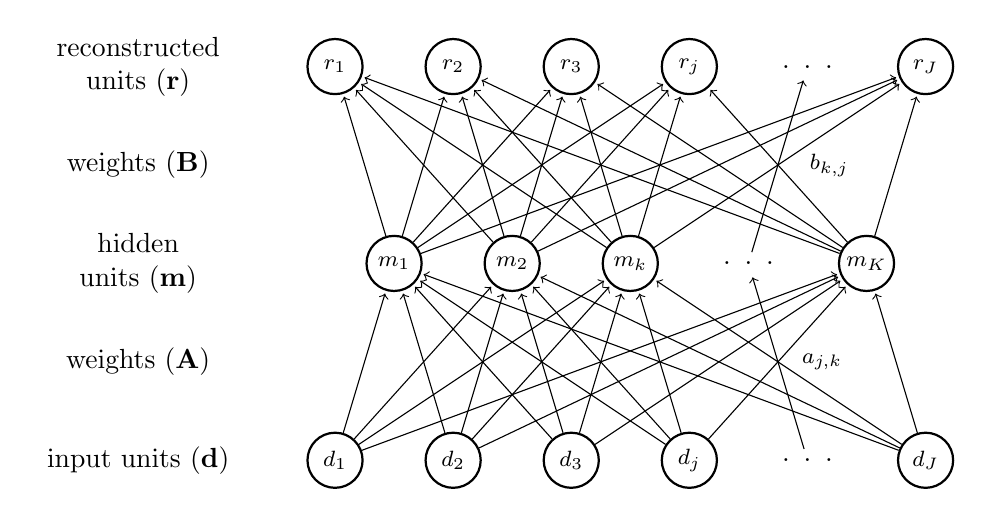
\begin{tikzpicture}[shorten >=1pt,->,draw=black!100]
	\def \rowtwoht{5cm}
	\def \weightstwo{3.75cm}
	\def \rowoneht{2.5cm}
	\def \weightsone{1.25cm}
	\def \basement{0cm}
	\tikzstyle{m-node}=[circle,draw=black!100,thick,inner sep=0pt,minimum size=7mm]
	\tikzstyle{r-node}=[circle,draw=black!100,thick,inner sep=0pt,minimum size=7mm]
	\tikzstyle{d-node}=[circle,draw=black!100,thick,inner sep=0pt,minimum size=7mm]
	\tikzstyle{dots}=[text width=5ex, text centered]
	\tikzstyle{annot}=[text width=17ex, text centered]
	% labels
	\node[annot] (r-layer) at (0cm,\rowtwoht) {reconstructed units ($\mathbf{r}$)};
	\node[annot] (weights) at (0cm,\weightstwo) {weights ($\mathbf{B}$)};
	\node[annot] (hidden-layer) at (0cm,\rowoneht) {hidden units ($\mathbf{m}$)};
	\node[annot] (weights) at (0cm,\weightsone) {weights ($\mathbf{A}$)};
	\node[annot] (d-layer) at (0cm,\basement) {input units ($\mathbf{d}$)};
	
	\node[dots] 	(m3)	at (7.75cm,\rowoneht)	 	{. . .};
	\node[dots] 	(r4) 	at (8.5cm,\rowtwoht)   		{. . .};
	\node[dots] 	(d4) 	at (8.5cm,\basement)   		{. . .};
	
	\footnotesize
	% hidden layer
	\node[m-node] 	(m0)	at (3.25cm,\rowoneht)		{$m_1$};
	\node[m-node] 	(m1)	at (4.75cm,\rowoneht)		{$m_2$};
	\node[m-node] 	(m2)	at (6.25cm,\rowoneht)	 	{$m_k$};
	\node[m-node] 	(m4)	at (9.25cm,\rowoneht)	 	{$m_K$};
	
	% reconstructed vector
	\node[r-node] 	(r0)	at (2.5cm,\rowtwoht)		{$r_1$};
	\node[r-node] 	(r1)	at (4cm,\rowtwoht)		{$r_2$};
	\node[r-node] 	(r2)	at (5.5cm,\rowtwoht)	 	{$r_3$};
	\node[r-node] 	(r3)	at (7cm,\rowtwoht) 		{$r_j$};
	\node[r-node] 	(r5) 	at (10cm,\rowtwoht)   		{$r_J$};
	%\node[r-node] 	(r6) 	at (9.75cm,\rowoneht)   	{$r_J$};
	
	% data vector
	\node[d-node] 	(d0)	at (2.5cm,\basement)		{$d_1$};
	\node[d-node] 	(d1)	at (4cm,\basement)		{$d_2$};
	\node[d-node] 	(d2)	at (5.5cm,\basement)	 	{$d_3$};
	\node[d-node] 	(d3)	at (7cm,\basement) 		{$d_j$};
	\node[d-node] 	(d5) 	at (10cm,\basement)   		{$d_J$};
	%\node[d-node] 	(d6) 	at (9.75cm,\basement)   	{$d_J$};
	
	\path
		(d0)	edge	node	{}	(m0)
		(d0)	edge	node	{}	(m1)
		(d0)	edge	node	{}	(m2)
		%(d0)	edge	node	{}	(m3)
		(d0)	edge	node	{}	(m4)
		%	
		(d1)	edge	node	{}	(m0)
		(d1)	edge	node	{}	(m1)
		(d1)	edge	node	{}	(m2)
		%(d1)	edge	node	{}	(m3)
		(d1)	edge	node	{}	(m4)
		%
		(d2)	edge	node	{}	(m0)
		(d2)	edge	node	{}	(m1)
		(d2)	edge	node	{}	(m2)
		(d2)	edge	node	{}	(m4)
		%
		(d3)	edge	node	{}	(m0)
		(d3)	edge	node	{}	(m1)
		(d3)	edge	node	{}	(m2)
		(d3)	edge	node	{}	(m4)
		%
		(d4)	edge	node[right=2mm]	{$a_{j,k}$}	(m3)
		%
		(d5)	edge	node	{}	(m0)
		(d5)	edge	node	{}	(m1)
		(d5)	edge	node	{}	(m2)
		(d5)	edge	node	{}	(m4)
	 
		(m0)	edge	node	{}	(r0)
		(m0)	edge	node	{}	(r1)
		(m0)	edge	node	{}	(r2)
		(m0)	edge	node	{}	(r3)
		(m0)	edge	node	{}	(r5)

		(m1)	edge	node	{}	(r0)
		(m1)	edge	node	{}	(r1)
		(m1)	edge	node	{}	(r2)
		(m1)	edge	node	{}	(r3)
		(m1)	edge	node	{}	(r5)

		(m2)	edge	node	{}	(r0)
		(m2)	edge	node	{}	(r1)
		(m2)	edge	node	{}	(r2)
		(m2)	edge	node	{}	(r3)
		(m2)	edge	node	{}	(r5)

		(m3)	edge	node[right=3mm]	{$b_{k,j}$}	(r4)	
		
		(m4)	edge	node	{}	(r0)
		(m4)	edge	node	{}	(r1)
		(m4)	edge	node	{}	(r2)
		(m4)	edge	node	{}	(r3)
		(m4)	edge	node	{}	(r5);
		
\end{tikzpicture}
\end{center}
\caption{many-to-many}
%: an input layer ($\mathbf{d}$), a hidden layer ($\mathbf{m}$), and an output layer
\label{fig:autoencoder}
\end{figure}

This is illustrated in fig.~\ref{fig:mcmm}, where $\mathbf{m}$ is the vector of hidden units, and $\mathbf{r}$ the vector of (reconstructed) surface units.
The hidden units are connected to surface units by a matrix of weights $\mathbf{C}$. 
Each individual arc $c_{j,k}$ has a value in $[0,1]$ that represents the weight on the connection between
$m_k$ and $r_j$.
Each node, i.e., each hidden unit and each surface unit, has an activity value in $[0,1]$ that
%Each hidden unit has an activity value in $[0,1]$ 
indicates whether it is \textsc{on} (active) or \textsc{off} (inactive).
The activity of $r_j$ is determined by a \emph{mixing function}, which takes as inputs the hidden-unit activities $\mathbf{m}$ and their respective weights $\mathbf{c}_j$
(section~\ref{sec:mixing-function}).

%Both hidden nodes and surface nodes have activity values, i.e., values in $[0,1]$ that
%indicate whether a node is \textsc{on} (active) or \textsc{off} (inactive). Each surface-node activity 
%is a function of the hidden-node activities and the weights that connect the hidden nodes to the surface node in question.

%Each surface node is either \textsc{on} (active) or \textsc{off} (inactive) depending 
%on the hidden-node activities and
%the weights connecting hidden nodes to surface nodes. 

%\subsection{Architecture}
%\label{subsec:architecture}

An MCMM can be viewed as a variant of the classical autoencoder
network \citep{dayan-and-zemel:95}, a type of neural network used for
unsupervised learning.  In autoencoders, a hidden layer is forced to
learn a compression scheme, i.e., a lower-dimensional encoding, for
a dataset.
 
%MCMMs are called \emph{Multiple Cause} Mixture Models because more
%than one hidden unit can take part in the activation of a surface
%unit.  
%This is illustrated in figure \ref{fig:mcmm}, where the nodes
%$\mathbf{m}$ are the hidden units, and $\mathbf{r}$ is the (reconstructed) surface
%vector.
%Each arc $c_{j,k}$ represents the weight on the connection between
%$m_k$ and $r_j$.
%The activity of $r_j$ is determined by a mixing function 
%(section~\ref{sec:mixing-function}).

\begin{figure*}[htb]
\begin{center}
\small
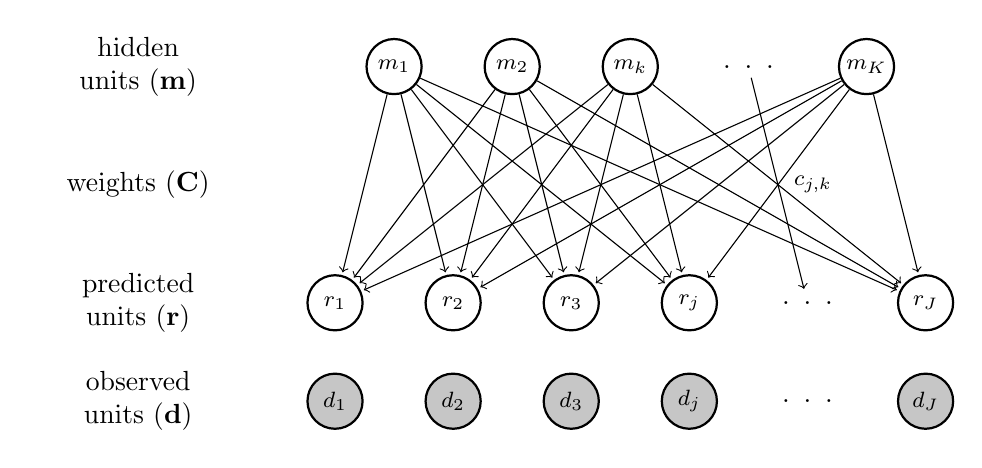
\begin{tikzpicture}[shorten >=1pt,->,draw=black!100]
	\def \rowtwoht{4.25cm}
	\def \weightlevel{2.75cm}
	\def \rowoneht{1.25cm}
	\def \basement{0cm}
	\tikzstyle{m-node}=[circle,draw=black!100,thick,inner sep=0pt,minimum size=7mm]
	\tikzstyle{r-node}=[circle,draw=black!100,thick,inner sep=0pt,minimum size=7mm]
	\tikzstyle{d-node}=[circle,draw=black!100,fill=gray!45,thick,inner sep=0pt,minimum size=7mm]
	\tikzstyle{dots}=[text width=5ex, text centered]
	\tikzstyle{annot}=[text width=17ex, text centered]
	% labels
	\node[annot] (hidden-layer) at (0cm,\rowtwoht) {hidden units ($\mathbf{m}$)};
	\node[annot] (weights) at (0cm,\weightlevel) {weights ($\mathbf{C}$)};
	\node[annot] (r-layer) at (0cm,\rowoneht) {predicted units ($\mathbf{r}$)};
	\node[annot] (d-layer) at (0cm,\basement) {observed units ($\mathbf{d}$)};
	
	\node[dots] 	(m3)	at (7.75cm,\rowtwoht)	 	{. . .};
	\node[dots] 	(r4) 	at (8.5cm,\rowoneht)   		{. . .};
	\node[dots] 	(d4) 	at (8.5cm,\basement)   		{. . .};
	
	\footnotesize
	% hidden layer
	\node[m-node] 	(m0)	at (3.25cm,\rowtwoht)		{$m_1$};
	\node[m-node] 	(m1)	at (4.75cm,\rowtwoht)		{$m_2$};
	\node[m-node] 	(m2)	at (6.25cm,\rowtwoht)	 	{$m_k$};
	\node[m-node] 	(m4)	at (9.25cm,\rowtwoht)	 	{$m_K$};
	
	% reconstructed vector
	\node[r-node] 	(r0)	at (2.5cm,\rowoneht)		{$r_1$};
	\node[r-node] 	(r1)	at (4cm,\rowoneht)		{$r_2$};
	\node[r-node] 	(r2)	at (5.5cm,\rowoneht)	 	{$r_3$};
	\node[r-node] 	(r3)	at (7cm,\rowoneht) 		{$r_j$};
	\node[r-node] 	(r5) 	at (10cm,\rowoneht)   		{$r_J$};
	%\node[r-node] 	(r6) 	at (9.75cm,\rowoneht)   	{$r_J$};
	
	% data vector
	\node[d-node] 	(d0)	at (2.5cm,\basement)		{$d_1$};
	\node[d-node] 	(d1)	at (4cm,\basement)		{$d_2$};
	\node[d-node] 	(d2)	at (5.5cm,\basement)	 	{$d_3$};
	\node[d-node] 	(d3)	at (7cm,\basement) 		{$d_j$};
	\node[d-node] 	(d5) 	at (10cm,\basement)   		{$d_J$};
	%\node[d-node] 	(d6) 	at (9.75cm,\basement)   	{$d_J$};
	
	\path 
		(m0)	edge	node	{}	(r0)
		(m0)	edge	node	{}	(r1)
		(m0)	edge	node	{}	(r2)
		(m0)	edge	node	{}	(r3)
		(m0)	edge	node	{}	(r5)
		(m1)	edge	node	{}	(r0)
		(m1)	edge	node	{}	(r1)
		(m1)	edge	node	{}	(r2)
		(m1)	edge	node	{}	(r3)
		(m1)	edge	node	{}	(r5)
		(m2)	edge	node	{}	(r0)
		(m2)	edge	node	{}	(r1)
		(m2)	edge	node	{}	(r2)
		(m2)	edge	node	{}	(r3)
		(m2)	edge	node	{}	(r5)
		(m3)	edge	node[right=1mm]	{$c_{j,k}$}	(r4)
		%	
		(m4)	edge	node	{}	(r0)
		(m4)	edge	node	{}	(r1)
		(m4)	edge	node	{}	(r2)
		(m4)	edge	node	{}	(r3)
		(m4)	edge	node	{}	(r5);
		
\end{tikzpicture}
\end{center}
\caption{Architecture of a Multiple Cause Mixture Model (MCMM)} 
\label{fig:mcmm}
\end{figure*}

%The MCMM learns by comparing the reconstructed vector $\mathbf{r}_i$ 
%to its corresponding original datapoint $\mathbf{d}_i$. The discrepancy between
%the two is quantified by an \emph{objective function}. 
%If there is a discrepancy, the values of the nodes in
%$\mathbf{m}_i$ as well as the weights $\mathbf{C}$ are adjusted 
%in order to reduce the discrepancy as much as possible.
%See section~\ref{sec:mcmm-learning} for more on the learning process.

%Suppose data points $\mathbf{d}_u$ and $\mathbf{d}_v$ have some features in common.
%Then, as the MCMM tries to reconstruct them in $\mathbf{r}_u$ and $\mathbf{r}_v$, respectively,
%similarities will emerge between their respective hidden-layer vectors $\mathbf{m}_u$ and $\mathbf{m}_v$.
%In particular, the vectors $\mathbf{m}_u$ and
%$\mathbf{m}_v$ should come to share at least one active node, i.e., at least
%one $k \in K$ such that $m_{u,k} = 1$ and $m_{v,k} = 1$.
%This can serve as a basis for clustering;
%i.e., $m_{i,k}$ indicates whether $\mathbf{d}_i$ is a member of cluster $k$.
		
\section{Mixing Function}
\label{ch4:sec:mixing-function}

The mapping between the layer of hidden nodes $\mathbf{m}$ 
and the layer of surface nodes $\mathbf{r}$ is governed by a 
\emph{mixing function}, which is essentially
a voting rule \citep{saund:94}; it maps from a set of (weighted)
input ``votes'' to a single output decision.  The output decision is 
an activity value for a particular surface-layer node. We will call the input votes
\emph{causes}. 

Each cause is a product of the form $m_{i,k} c_{j,k}$ for $k \in K$.
There are thus a total of $K$ distinct causes for a given surface node $r_{i,j}$. 
If the cause $m_{i,h} c_{j,h}$, where $h \in K$, is equal to $1$ or surpasses some
threshold, then $m_{i,h} c_{j,h}$ is an \emph{active cause}.
%The input votes, are the activities of the hidden nodes,
%i.e., the $K$-length vector $\mathbf{m}_i$,
%coupled with their respective weights, i.e., the $K$-length vector 
%$\mathbf{c}_j$. 
Any differentiable function
that maps from the vector pair $(\mathbf{m}_i, \mathbf{c}_j)$ 
to an activity value for $r_{i,j}$ can in theory serve as a mixing function. 
There are thus an infinite number of theoretically possible mixing functions.

%Following \cite{saund:94}, we use the 
%There are perhaps an infinite number of possible mixing functions. 
%Any function that maps from a set of votes 
%(and their respective weights) to a single output decision will suffice.
One possibility is the \textbf{Noisy-OR} function:
 \begin{equation}\label{eq:noisy-or}
  r_{i,j} = 1 - \prod\limits_{k} (1 - m_{i,k} c_{j,k})
 \end{equation}
% We will call the inputs to the Noisy-OR function \emph{causes}. Each cause is a product of the form $m_{i,k} c_{j,k}$. 
 The Noisy-OR function acts as a kind of \textit{OR} gate, or, to put it another way, an``at-least-one" gate. That is, the surface node $r_{i,j}$ is $1$ as long as \emph{at least one} cause is active.
 % (i.e., $m_{i,k} c_{j,k} = 1$ for at least one $k$ in $K$). 
 If two or more causes are active,
%$1$ (or $\ge$ than a threshold), 
$r_{i,j}$ is still going to be $1$. The output of Noisy-OR does not change as the number of active causes change, as long as there is at least one active cause.

Another possible mixing function is the \textbf{sigmoidal weighted sum}, the composition of the sigmoid function $S$ and the function $t_{i,j}$, which computes a weighted sum, i.e., the inner product of the cluster-activity vector $\mathbf{m}_i$ and the weight vector $\mathbf{c}_j$:

	\begin{align} %\label{eq:sigws}
	\label{eq:sig}
	r_{i,j} = S(t_{i,j}) &= \frac{1}{1 + e^{-t_{i,j}}} \quad %\\   %\qquad \text{where} \quad
	%\label{eq:ws}
	\text{where} \quad t_{i,j} = \sum_k m_{i,k} c_{j,k}
	\end{align}
This is the mixing (or activation) function that is typically used in classical autoencoders. 
Whereas the output of Noisy-OR is independent of the number of active causes (as long as there is at least one), the output of \eqref{eq:sig} DOES change with the number of active causes: The value $t_{i,j} = \sum_k m_{i,k} c_{j,k}$ is clearly going to increase as the number of active clusters increases.
%(i.e., products of the form $m_{i,k} c_{j,k}$ that equal $1$ or are greater than some threshold) 
As $t_{i,j}$ increases, $S(t_{i,j})$ will get closer to $1$; as %it
$t_{i,j}$ 
decreases, $S(t_{i,j})$ will get closer to $0$.


\section{Learning}
\label{ch4:sec:learning}
%\label{autoencoder-learning}

% A data compression scheme is useful only to the extent that it allows
% for the recovery of the source data from the compressed
% representations. In autoencoder terms, this means that 

%The reconstruction layer attempts to
%decode the hidden layer's representations and
In both the classical autoencoder and the MCMM, learning occurs as a
result of the algorithm's search for an optimal valuation of key variables (e.g., weights), 
i.e., a valuation that minimizes %or maximizes an the
%\emph{reconstruction error} $E$, 
the discrepancy between
reconstructed and original data points.  The search is conducted
via %some method of 
numerical optimization; we use the nonlinear conjugate gradient method.
%gradient-based technique, e.g., gradient descent or
%the conjugate gradient method.
%
Our objective function is a simple error function, namely the
normalized sum of squares error:
\begin{equation}
E = \frac{1}{I \times J} \sum_{i} \sum_{j} {(r_{i,j} - d_{i,j})}^2
\end{equation}
 where $I \times J$ is the total number of features in the dataset.
The MCMM's task is to minimize this function by adjusting the
 values in $\mathbf{M}$ and $\mathbf{C}$, where
 %$I \times $ matrix $\mathbf{M}$ and the $J \times K$ matrix $\mathbf{C}$.
$\mathbf{M}$ is the $I \times K$ matrix that
% of dimensions $I \times K$,
encodes each data point's cluster-activity vector, 
and $\mathbf{C}$ is the $J \times K$ matrix that
%, of dimensions $J \times K$, 
encodes the weights between $\mathbf{m}_i$ and $\mathbf{r}_i$ for every $i \in I$ (see fig.~\ref{fig:example}). 
%$\mathbf{C}$ can also be interpreted as encoding the cluster centroids 
%(the clusters' ``average'' data points).
%Each column in $\mathbf{C}$ is in effect a feature vector; the $k^{\text{th}}$ column is 
%the $k^{\text{th}}$ cluster's average feature vector.
% \begin{align*}
% 	% E &= \frac{1}{I} \sum_{i} e_{i} \\
% 	% e_{i} &= \frac{1}{J} \sum_{j} {(r_{i,j} - d_{i,j})}^2
% 	E &= \frac{1}{I \times J} \sum_{i} \sum_{j} {(r_{i,j} - d_{i,j})}^2
% \end{align*}
% %\marginpar{Rationale for normalized SSE?} 
% which is minimized.
% rather than maximized.  


%; our techniques are described in section~\ref{subsec:objfunc}.
% There are a number of possibilities regarding the particular error
% function and gradient-based technique. We describe our choices in
% section~\ref{subsec:objfunc}.
% Any information loss in the compression will result in reconstructed
% vectors that differ from the original data points.  This is called
%the \emph{reconstruction error} is measured by some error function
%$err$, such as the
%%.  A typical error function is 
%the sum of squared error ($err_i = \sum_{j}{(d_{i,j} -
%  r_{i,j})}^2$). The global reconstruction error $E$, for the whole
%dataset, is the sum of all $err_i$.
%% over $i \in I$.
%%
%To discover a compression scheme with a minimal $E$, autoencoders
%use gradient-based search techniques, e.g., gradient descent or the
%conjugate gradient method.  We describe our error function in
%section~\ref{subsec:objfunc}.

% The autoencoder's goal is to discover a compression scheme that causes a minimal $E$, 
% and since $E$ is ultimately a function of $\mathbf{A}$ and $\mathbf{B}$, 
% this task reduces to finding the valuations for $\mathbf{A}$ and $\mathbf{B}$ that minimize $E(\mathbf{A},\mathbf{B}$). To this end, autoencoders use gradient-based search techniques, e.g., gradient descent or the conjugate gradient method. In the remainder of this section, we provide a very general description of an autoencoder's weight updating process. The details, especially the specific form of the weight-update function, depend on the particular gradient-based technique used. 

% Taking as input the data points $\mathbf{d}_i \in \mathbf{D}$, the network yields a reconstructed vector $\mathbf{r}_i$ for each individual $\mathbf{d}_i$. Because $\mathbf{D}$ contains $I$ data points, one epoch (i.e., one cycle through the dataset) is complete after $I$ iterations, whereupon ${E}(\mathbf{A}, \mathbf{B})$ is calculated, and each weight in $\mathbf{A}$ and $\mathbf{B}$ is adjusted in a way that furthers the descent of $E$ toward a minimum. 
% In particular, the algorithm adds to each 
% $b_{k,j} \in \mathbf{B}$ a quantity proportional to the negative gradient of 
% $E$ at $b_{k,j}$, or $-\frac{\partial E}{\partial b_{k,j}}$. 
% It similarly adds to each $a_{j,k} \in \mathbf{A}$
% a quantity proportional to the negative gradient of $E$ at $a_{j,k}$,
% or $-\frac{\partial E}{\partial a_{j,k}}$.
% These weight updates serve to improve the network's compression model, so that each successive epoch yields a smaller reconstruction error than the preceding epoch.
% The succession of epochs continues until $E$ falls below some small predesignated value.


% \subsection{The MCMM as an autoencoder variant}
% \label{subsec:mcmm-variant}

%\subsubsection{Architecture}
% Like the classical autoencoder, the MCMM has a hidden layer $\mathbf{m}$ and a reconstruction layer $\mathbf{r}$, as illustrated in figure \ref{fig:mcmm}. 
% However, the MCMM does not have an explicit
% data (or input) layer corresponding to the classical autoencoder's $\mathbf{d}$.
% Because the MCMM has only a two layers of nodes instead of three, it needs only a single layer of connecting weights, namely the weight matrix $\mathbf{C}$. This is a $J \times K$ matrix,
% since there are $K$ nodes in $\mathbf{m}$ and $J$ nodes in $\mathbf{r}$,
% and every $m_k$ must be linked to every $r_j$.

%\subsubsection{Mixing Function}
% MCMMs are distinguished by their propensity for learning hidden-unit activations and weight configurations that have clear interpretations.

% In the classical autoencoder, the activity $\phi(net)$ of any node $y$ is a
% function of its net raw input $net_y$, which is the weighted sum of $y$'s
% individual input signals (see \eqref{weighted-sum}). 
% The logistic sigmoid function $\phi$ then scales ${net}_y$ so that it falls within $[0,1]$.

% \begin{align*}
% r_{j} &= \sigma({net}_j) \\
% &= \sigma\big(\sum_k b_{k,j} \cdot m_k \big) \\
% &= \sigma \bigg(\sum_k b_{k,j} \cdot \sigma \big({net}_k \big) \bigg) \\
% &= \sigma \bigg(\sum_k b_{k,j} \cdot \sigma \big(\sum_j a_{j,k} \cdot d_j \big) \bigg) \\
% \end{align*}
% The activity of any given reconstruction node $r_j$ depends not only on the weights $\mathbf{B}$, but also on the weights $\mathbf{A}$.
% Moreover, $\mathbf{A}$ and $\mathbf{B}$ may differ.
% When $\mathbf{A} \ne \mathbf{B}$, the $\mathbf{B}$ weights can counteract the effects of the $\mathbf{A}$ weights, giving rise to unexpected activities among the $\mathbf{m}$ units and obscuring the  
% relationships between the $\mathbf{m}$ units and the $\mathbf{r}$ units.

% The MCMM, in contrast, is designed with the express purpose of providing a coherent causal explanation for regularities in surface data.
% What makes this possible?
% \begin{itemize} 
% \item \textit{Binary activities and weights.} Both the weights and the hidden unit activities are constrained to stay in $[0,1]$. At convergence, moreover, all values---both weights and hidden activities---should be either $0$ or $1$. \textit{Why is this important?} Binary values, i.e., \textsc{true} and \textsc{false}, have clear interpretations.
% \item \textit{Single layer of weights.} An MCMM has only one layer of weights. \textit{Why is this important?} The activities of the hidden units are manipulated directly in response to the reconstruction error.
% \item 
% \textit{How so?} In the classical autoencoder, the terms $m_kc_{j,k}, k \in K$ are combined linearly prior to sigmoid squashing. But MCMMs employ mixing functions such that the combination of these terms is nonlinear from the start. \textit{Why does this matter?} This ``total" nonlinearity encourages (?) weights to converge toward discrete values. The ultimate decision is then based on multiple discrete, either-or votes.
% \textit{Why, then, is clipping necessary?}
% \end{itemize}

% The classical autoencoder's activation function $\sigma({net}_y)$ is one possible mixing function,
% for it indeed takes the $K$ distinct input signals to node $y$ and yields a single activity value.
% However, as Saund points out, $\sigma({net}_y)$ is not well suited to the purpose of coherently distinguishing causes from non-causes. This is because $net_y$ is additive rather than multiplicative. Noisy-or is multiplicative:
% \begin{align*}
% r_{j} &= 1 - (1 - m_0c_{0,j}) \times (1 - m_1c_{1,j}) \times (1 - m_2c_{2,j}) \\
% &= 1 - (1 - 0) \times (1 - 0) \times (1 - 1) \\ 
% &= 1 - 1 \times 1 \times 0 \\
% &= 1
% \end{align*}
% As long as at least one $m_kc_{j,k} = 1$ (where $k = 0,1,\dots,K$), $r_{j}$ will be active,
% and $r_{j} = 0$ only if all products $m_kc_{j,k}$ are zero.
% Notice that $m_kc_{j,k} = 1$ only if both $m_k = 1$ and $c_{j,k} = 1$.
% On the other hand, with sigmoid squashing, $\sigma({net}_j)$ is never truly zero; it just gets infinitely close to zero.
% And $\sigma({net}_j)$ will be close to $1$ as long as ${net}_j = \sum_K m_k c_{j,k}$ is sufficiently large. 
% There are an infinite number of valuations for $\mathbf{m}$ and $\mathbf{c}_{j}$ that could give rise to a sufficiently large ${net}_j$.

% The function ${net}$ is an example of a linear mixing function. However, the autoencoder's mixing function
% is made nonlinear by $\phi({net}_y)$, which ``squashes" $net_y$ to fall within $[0,1]$.

%\subsubsection{Learning}
%\label{mcmm-learning}

%\paragraph{MCMM}

%\marginpar{MD: In fig.~\ref{fig:example}, we use $\mathbf{M}$, but
%  in previous figures we use $\mathbf{m}$.  Also, why is it sometimes
%  $\mathbf{m_k}$ and sometimes $\mathbf{m_{i,k}}$?  ($i$ refers to the
%  $i^{\text{th}}$ word?)}

The MCMM's learning process is similar to Expectation Maximization
(EM) in that at any given time it holds one set of variables 
fixed while optimizing the other set. We thus have two functions, \textsc{Optimize-M}
and \textsc{Optimize-C}, which take turns optimizing their respective matrices.
% However, if the algorithm is to optimize $\mathbf{M}$, it must first
% know $\mathbf{C}$, and vice versa.  Therefore, the algorithm can only
% focus on matrix at time, optimizing the one while holding the other
% fixed.
% The learning process consists of two distinct optimization
% functions:
%, \textsc{Optimize-M} and \textsc{Optimize-C}.
%\begin{description}
%\item[
% \textsc{Optimize-M} holds $\mathbf{C}$ fixed in order to optimize the
% cluster activity vectors in $\mathbf{M}$, while \textsc{Optimize-C}
% holds $\mathbf{M}$ fixed in order to optimize the cluster centroids in
% $\mathbf{C}$.
%\end{description}

The function \textsc{Optimize-M} visits each of the $I$ cluster-activity vectors $\mathbf{m}_i$ in
$\mathbf{M}$, optimizing each one separately.
%, one at a time.
%in $\mathbf{M}$, 
For each $\mathbf{m}_i$, \textsc{Optimize-M} enters an optimization 
loop over its $K$ components, adjusting each 
$m_{i,k}$ by a
quantity proportional to the negative gradient of $E$ at $m_{i,k}$. \marginpar{How is this proportion determined?} 
This loop repeats until $E$
ceases to decrease significantly,
whereupon \textsc{Optimize-M} proceeds to the next $\mathbf{m}_i$.  
The function \textsc{Optimize-C} consists of a single optimization loop over the 
entire matrix
$\mathbf{C}$. Each $c_{j,k}$ is adjusted by a quantity
proportional to the negative gradient of $E$ at $c_{j,k}$.
%, or $-\frac{\partial E}{\partial c_{j,k}}$.
%(in the case of gradient descent).  
%Since $E$ is simply
%$\sum_i e_i$, i.e., the sum of the errors of the individual data-point
%reconstructions, $-\frac{\partial E}{\partial c_{j,k}} = -\sum_i
%\frac{\partial e_i}{\partial c_{j,k}}$.  Thus, the adjustment to each
%$c_{j,k}$ takes into account the error of each reconstructed vector
%$\mathbf{r}_i$ in $\mathbf{R}$. However,
Unlike \textsc{Optimize-M}, which comprises $I$ separate optimization
loops, \textsc{Optimize-C} consists of just one, 
%optimizing the $\mathbf{C}$ matrix as a whole.  
When each of its $J \times K$
components has been adjusted, one round of updates to $\mathbf{C}$ is
complete.  $E$ is reassessed only between completed rounds of
updates. If the change in $E$ remains significant, another round begins.  
Both \textsc{Optimize-M} and \textsc{Optimize-C} are enclosed within 
an ``alternation loop" 
that alternates between the two functions, holding $\mathbf{C}$ fixed
during \textsc{Optimize-M}, and vice versa.
This alternation continues until $E$ cannot be decreased further. At
this point, an ``outer loop''
splits the cluster which contributes the most to the error, adds one
to the cluster count $K$, and restarts the alternation loop. The outer loop
repeats until it reaches an overall stopping criterion, e.g., $E = 0$.
%; otherwise, the function terminates.
 \subsection{Bound Constrained Optimization}
The optimization task is subject to the constraint %$0 le m_{i,k} ge 1$
that no value in $\mathbf{M}$ or $\mathbf{C}$ may exceed 1 or fall below 0. In other words,
it is a task of bound constrained optimization. Thus, whenever a value in either $\mathbf{M}$ or $\mathbf{C}$ is about
to fall below 0, it is set to 0. Likewise, whenever a value is about to exceed 1, it is set to 1
\citep{ni:yuan:1997}.
 %It repeatedly iterates over the $J \times K$ components of $\mathbf{C}$, stopping only when it finds a local minimum of $E$ is
  
%What is the inner loop and what is the outer loop?
%There are actually two inner loops: Opt-M is immediately followed by Opt-C. These two are encapsulated within a larger outer loop.
%What is the stopping criterion for the inner loop? What happens when this criterion is met?
%What is the stopping criterion for the outer loop?
%Cluster Splitting. Where does this enter the narrative?
%At this point, the algorithm then finds the worst cluster among the currently existing clusters and splits it, thereby increasing the cluster count $K$ by one.

\subsection{A Simple MCMM Example}
\label{subsec:example}

Fig.~\ref{fig:example} shows an example of an MCMM for two data points (i.e., $I = 2$).
The hidden cluster activities $\mathbf{M}$, the weights $\mathbf{C}$,
and the mixing function $r$ constitute a model that reproduces the
observed data points $\mathbf{D}$.
%
%\marginpar{MD: I don't quite understand the ``center vector''
  %statement}
%
The nodes $m_{i,k}$ represent cluster activities; if $m_{1,2} = 1$,
for instance, the second cluster is active for $\mathbf{d}_1$ (i.e.,
$\mathbf{d}_1$ is a member of cluster 2).
%
Note that the $J \times K$ weight matrix $\mathbf{C}$ is the same for
all data points, and
%
% For each data point, the arcs emanating from cluster
% 1 and cluster 2 represent the components of $\mathbf{C}$'s first and
% second rows, respectively. The $k$th row in $\mathbf{C}$ is thus
% uniquely associated with the $k$th cluster. Moreover, 
%
the $k^{\text{th}}$ row in $\mathbf{C}$ can be seen as the $k^{\text{th}}$
cluster's ``average" vector: the $j^{\text{th}}$ component in
$\mathbf{c}_k$ is 1 only if all data points in cluster $k$ have
1 at feature $j$.
%the $k^{\text{th}}$ row of $\mathbf{C}$ is in effect
%the center vector of the $k^{\text{th}}$ hidden cluster.
%
%In the figure, 

%\begin{figure}[htb!]
%\usetikzlibrary{positioning}
%%\begin{minipage}{.3\textwidth}
%\begin{center}
%%\subfigure[Learning in Progress]{
%\begin{tikzpicture}[shorten >=1pt,->,draw=black!100, scale=0.85]
%	\footnotesize
%%	\def \attic{5.95cm}
%%	\def \rowtwoht{5.4cm}
%%	\def \weightlevel{3.9cm}
%%	\def \rowoneht{2.4cm}
%%	\def \basement{1.8cm}
%%	\def \data{1cm}
%%	\def \china{0cm}
%
%	\def \attic{5.4cm}
%	\def \rowtwoht{4.8cm}
%	\def \weightlevel{3.6cm}
%	\def \rowoneht{2.4cm}
%	\def \basement{1.8cm}
%	\def \data{1cm}
%	\def \china{0cm}
%		
%	\tikzstyle{m-node}=[circle,draw=black!100,thick,inner sep=0pt,minimum size=6mm]
%	\tikzstyle{r-node}=[circle,draw=black!100,thick,inner sep=0pt,minimum size=6mm]
%	\tikzstyle{d-node}=[circle,draw=black!100,fill=gray!45,thick,inner sep=0pt,minimum size=6mm]
%	%\tikzstyle{dots}=[text width=5ex, text centered]
%	\tikzstyle{annot}=[text width=2.5em]
%	% labels
%	\tikzstyle{label}=[text width=2.5em, text centered]
%	\tikzstyle{formula}=[text width=30em, text centered]
%	
%	\scriptsize
%	\node[annot] (hidden-layer) at (0cm,\rowtwoht) {$\mathbf{M}_{(i,k)}$};
%	\node[annot] (weights) at (0cm,\weightlevel) {$\mathbf{C}_{(j,k)}$};
%	\node[annot] (r-layer) at (0cm,\rowoneht) {$\mathbf{R}_{(i,j)}$};
%	
%	% hidden layer
%	\scriptsize
%	\node[m-node] 	(ma00)	at (1.45cm,\rowtwoht)		{$.2$};
%	\node[m-node] 	(ma01)	at (3.35cm,\rowtwoht)		{$.9$};
%	\node[m-node] 	(ma10)	at (5.55cm,\rowtwoht) 	{$.8$};
%	\node[m-node] 	(ma11)	at (7.45cm,\rowtwoht)	 	{$.1$};
%	% \node[m-node] 	(m20)	at (9.65cm,\rowtwoht) 	{$.8$};
%	% \node[m-node] 	(m21)	at (11.55cm,\rowtwoht)	 	{$.9$};
%	
%	%\footnotesize
%	\node[label]	(ml00) 	at (1.45cm,\attic)		{$m_{1,1}$}; %1.75 -> 1.45
%	\node[label]	(ml01) 	at (3.35cm,\attic)		{$m_{1,2}$}; %3.05 -> 3.35
%	\node[label] 	(ml10)	at (5.55cm,\attic) 	{$m_{2,1}$};     %5.85 -> 5.55
%	\node[label] 	(ml11)	at (7.45cm,\attic)	 	{$m_{2,2}$}; %7.15 -> 7.45
%	% \node[label] 	(ml20)	at (9.65cm,\attic) 	{$m_{3,1}$};     %9.95 -> 9.65
%	% \node[label] 	(ml21)	at (11.55cm,\attic)	 	{$m_{3,2}$}; %11.25 -> 11.55
%	
%	\scriptsize
%	\node[r-node] 	(ra00)	at (1.1cm,\rowoneht)		{$.24$};
%	\node[r-node] 	(ra01)	at (2.4cm,\rowoneht)		{$.81$};
%	\node[r-node] 	(ra02)	at (3.7cm,\rowoneht)	 	{$.23$};
%	
%	\node[r-node] 	(ra10)	at (5.2cm,\rowoneht) 		{$.68$};
%	\node[r-node] 	(ra11) 	at (6.5cm,\rowoneht)   	{$.16$};
%	\node[r-node] 	(ra12)	at (7.8cm,\rowoneht)		{$.76$};
%	
%	% \node[r-node] 	(r20) 	at (9.3cm,\rowoneht)  		{$.71$};
%	% \node[r-node] 	(r21)	at (10.6cm,\rowoneht) 		{$.83$};
%	% \node[r-node] 	(r22) 	at (11.9cm,\rowoneht)   	{$.77$};
%	
%	\node[label] 	(rl00)	at (1.1cm,\basement)		{$r_{1,1}$};
%	\node[label] 	(rl01)	at (2.4cm,\basement)		{$r_{1,2}$};
%	\node[label] 	(rl02)	at (3.7cm,\basement)	 	{$r_{1,3}$};
%	
%	\node[label] 	(rl10)	at (5.2cm,\basement) 		{$r_{2,1}$};
%	\node[label] 	(rl11) 	at (6.5cm,\basement)   	{$r_{2,2}$};
%	\node[label] 	(rl12)	at (7.8cm,\basement)		{$r_{2,3}$};
%	
%%	\node[label] 	(rl20) 	at (9.3cm,\basement)  		{$r_{3,1}$};
%%	\node[label] 	(rl21)	at (10.6cm,\basement) 		{$r_{3,2}$};
%%	\node[label] 	(rl22) 	at (11.9cm,\basement)   	{$r_{3,3}$};
%
%	\draw[-] (4.45cm, \attic+1.5mm) -- (4.45cm, \basement-1.5mm);
%%	\draw[-] (8.55cm, \attic+1.5mm) -- (8.55cm, \basement-1.5mm);
%
%	\scriptsize
%	\path
%		(ma00)	edge	node [left]	{$.85$} (ra00)
%		(ma00)	edge	node [left,xshift=-1mm,yshift=3mm]	{$.1$}	(ra01)
%		(ma00)	edge	node [left,xshift=-1mm,yshift=8mm]	{$.95$}	(ra02)
%
%		(ma01)	edge	node [right,xshift=3mm,yshift=8mm]	{$.1$}	(ra00)
%		(ma01)	edge	node [right,xshift=1mm,yshift=3mm]	{$.9$}	(ra01)
%		(ma01)	edge	node [right]	{$.05$} (ra02)
%		%
%		(ma10)	edge	node [left] {$.85$} (ra10)
%		(ma10)	edge	node [left,xshift=-1mm,yshift=3mm]	{$.1$}	(ra11)
%		(ma10)	edge	node [left,xshift=-1mm,yshift=8mm] {$.95$}	(ra12)
%		
%		(ma11)	edge	node [right,xshift=3mm,yshift=8mm]	{$.1$}	(ra10)
%		(ma11)	edge	node [right,xshift=1mm,yshift=3mm]	{$.9$}	(ra11)
%		(ma11)	edge	node [right]	{$.05$} (ra12);
%		%
		% (m20)	edge	node [left]	{$.85$}	(r20)
		% (m20)	edge	node [left,xshift=-1mm,yshift=4mm]	{$.1$}	(r21)
		% (m20)	edge	node [left,xshift=-1mm,yshift=10mm]	{$.95$} (r22)
		
		% (m21)	edge	node [right,xshift=3mm,yshift=10mm]		{$.1$}	(r20)
		% (m21)	edge	node [right,xshift=1mm,yshift=4mm]{$.9$}	(r21)
		% (m21)	edge	node [right]	{$.05$}	(r22);		
		
%\end{tikzpicture}
%\label{fig:example:fig1}
%\caption{A simple MCMM example} % showing learning in progress}
%\label{fig:example:fig1}
%\end{center}
%\end{figure}

\begin{figure}[htb!]
\usetikzlibrary{positioning}
\begin{center}
\subfigure[Observed Data]{
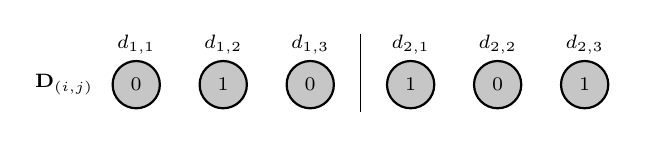
\begin{tikzpicture}[shorten >=1pt,->,draw=black!100, scale=0.85]
	\scriptsize
	\tikzstyle{label}=[text width=3em, text centered]
	\tikzstyle{annot}=[text width=2.5em]
	\tikzstyle{d-node}=[circle,draw=black!100,fill=gray!45,thick,inner sep=0pt,minimum size=6mm]
	
	\def \china{0.6cm}
	\def \data{0cm}
	
	\node[annot] (d-layer) at (0cm,\data) {$\mathbf{D}_{(i,j)}$};
	\draw[-] (4.45cm, \china+1.5mm) -- (4.45cm, \data-4.5mm);
%	\draw[-] (8.55cm, \china+1.5mm) -- (8.55cm, \data-4.5mm);
	%\draw[-] (-1cm, \china+.5cm) -- (13cm, \china+.5cm);
	%\draw[-] (-1cm, \data-.5cm) -- (13cm, \data-.5cm);
	
	\node[label] 	(dl00)	at (1.1cm,\china)		{$d_{1,1}$};
	\node[label] 	(dl01)	at (2.4cm,\china)		{$d_{1,2}$};
	\node[label] 	(dl02)	at (3.7cm,\china)	 	{$d_{1,3}$};
	
	\node[label] 	(dl10)	at (5.2cm,\china) 		{$d_{2,1}$};
	\node[label] 	(dl11) 	at (6.5cm,\china)   	{$d_{2,2}$};
	\node[label] 	(dl12)	at (7.8cm,\china)		{$d_{2,3}$};
	
	% \node[label] 	(dl20) 	at (9.3cm,\china)  		{$d_{3,1}$};
	% \node[label] 	(dl21)	at (10.6cm,\china) 		{$d_{3,2}$};
	% \node[label] 	(dl22) 	at (11.9cm,\china)   	{$d_{3,3}$};
	
	\node[d-node] 	(d00)	at (1.1cm,\data)		{$0$};
	\node[d-node] 	(d01)	at (2.4cm,\data)		{$1$};
	\node[d-node] 	(d02)	at (3.7cm,\data)		{$0$};

	\node[d-node] 	(d10)	at (5.2cm,\data)		{$1$};
	\node[d-node] 	(d11)	at (6.5cm,\data)		{$0$};
	\node[d-node] 	(d12)	at (7.8cm,\data)		{$1$};
	
	% \node[d-node] 	(d20)	at (9.3cm,\data)		{$1$};
	% \node[d-node] 	(d21)	at (10.6cm,\data)		{$1$};
	% \node[d-node] 	(d22)	at (11.9cm,\data)		{$1$};
\end{tikzpicture}
\label{fig:example:subfig0}
}
\end{center}

\usetikzlibrary{positioning}
%\begin{minipage}{.3\textwidth}
\begin{center}
\subfigure[Learning in Progress]{
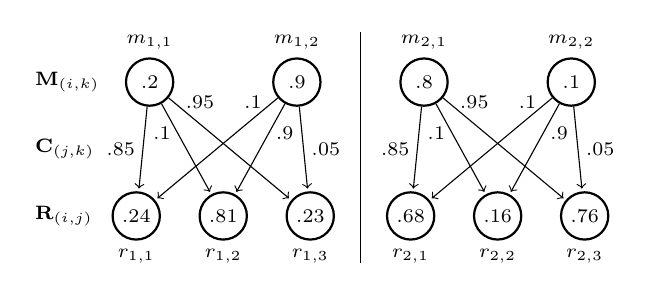
\begin{tikzpicture}[shorten >=1pt,->,draw=black!100, scale=0.85]
	\footnotesize
%	\def \attic{5.95cm}
%	\def \rowtwoht{5.4cm}
%	\def \weightlevel{3.9cm}
%	\def \rowoneht{2.4cm}
%	\def \basement{1.8cm}
%	\def \data{1cm}
%	\def \china{0cm}

	\def \attic{5cm}
	\def \rowtwoht{4.4cm}
	\def \weightlevel{3.4cm}
	\def \rowoneht{2.4cm}
	\def \basement{1.8cm}
	\def \data{1cm}
	\def \china{0cm}
		
	\tikzstyle{m-node}=[circle,draw=black!100,thick,inner sep=0pt,minimum size=6mm]
	\tikzstyle{r-node}=[circle,draw=black!100,thick,inner sep=0pt,minimum size=6mm]
	\tikzstyle{d-node}=[circle,draw=black!100,fill=gray!45,thick,inner sep=0pt,minimum size=6mm]
	%\tikzstyle{dots}=[text width=5ex, text centered]
	\tikzstyle{annot}=[text width=2.5em]
	% labels
	\tikzstyle{label}=[text width=2.5em, text centered]
	\tikzstyle{formula}=[text width=30em, text centered]
	
	\scriptsize
	\node[annot] (hidden-layer) at (0cm,\rowtwoht) {$\mathbf{M}_{(i,k)}$};
	\node[annot] (weights) at (0cm,\weightlevel) {$\mathbf{C}_{(j,k)}$};
	\node[annot] (r-layer) at (0cm,\rowoneht) {$\mathbf{R}_{(i,j)}$};
	
	% hidden layer
	\scriptsize
	\node[m-node] 	(ma00)	at (1.3cm,\rowtwoht)		{$.2$};
	\node[m-node] 	(ma01)	at (3.5cm,\rowtwoht)		{$.9$};
	\node[m-node] 	(ma10)	at (5.4cm,\rowtwoht) 	{$.8$};
	\node[m-node] 	(ma11)	at (7.6cm,\rowtwoht)	 	{$.1$};
	% \node[m-node] 	(m20)	at (9.65cm,\rowtwoht) 	{$.8$};
	% \node[m-node] 	(m21)	at (11.55cm,\rowtwoht)	 	{$.9$};
	
	%\footnotesize
	\node[label]	(ml00) 	at (1.3cm,\attic)		{$m_{1,1}$}; %1.75 -> 1.45
	\node[label]	(ml01) 	at (3.5cm,\attic)		{$m_{1,2}$}; %3.05 -> 3.35
	\node[label] 	(ml10)	at (5.4cm,\attic) 	{$m_{2,1}$};     %5.85 -> 5.55
	\node[label] 	(ml11)	at (7.6cm,\attic)	 	{$m_{2,2}$}; %7.15 -> 7.45
	% \node[label] 	(ml20)	at (9.65cm,\attic) 	{$m_{3,1}$};     %9.95 -> 9.65
	% \node[label] 	(ml21)	at (11.55cm,\attic)	 	{$m_{3,2}$}; %11.25 -> 11.55
	
	\scriptsize
	\node[r-node] 	(ra00)	at (1.1cm,\rowoneht)		{$.24$};
	\node[r-node] 	(ra01)	at (2.4cm,\rowoneht)		{$.81$};
	\node[r-node] 	(ra02)	at (3.7cm,\rowoneht)	 	{$.23$};
	
	\node[r-node] 	(ra10)	at (5.2cm,\rowoneht) 		{$.68$};
	\node[r-node] 	(ra11) 	at (6.5cm,\rowoneht)   	{$.16$};
	\node[r-node] 	(ra12)	at (7.8cm,\rowoneht)		{$.76$};
	
	\node[label] 	(rl00)	at (1.1cm,\basement)		{$r_{1,1}$};
	\node[label] 	(rl01)	at (2.4cm,\basement)		{$r_{1,2}$};
	\node[label] 	(rl02)	at (3.7cm,\basement)	 	{$r_{1,3}$};
	
	\node[label] 	(rl10)	at (5.2cm,\basement) 		{$r_{2,1}$};
	\node[label] 	(rl11) 	at (6.5cm,\basement)   	{$r_{2,2}$};
	\node[label] 	(rl12)	at (7.8cm,\basement)		{$r_{2,3}$};

	\draw[-] (4.45cm, \attic+1.5mm) -- (4.45cm, \basement-1.5mm);

	\scriptsize
	\path
		(ma00)	edge	node [left]	{$.85$} (ra00)
		(ma00)	edge	node [left,xshift=-1mm,yshift=2mm]	{$.1$}	(ra01)
		(ma00)	edge	node [left,xshift=-1mm,yshift=6mm]	{$.95$}	(ra02)

		(ma01)	edge	node [right,xshift=2.5mm,yshift=6mm]	{$.1$}	(ra00)
		(ma01)	edge	node [right,xshift=1mm,yshift=2mm]	{$.9$}	(ra01)
		(ma01)	edge	node [right]	{$.05$} (ra02)
		%
		(ma10)	edge	node [left] {$.85$} (ra10)
		(ma10)	edge	node [left,xshift=-1mm,yshift=2mm]	{$.1$}	(ra11)
		(ma10)	edge	node [left,xshift=-1mm,yshift=6mm] {$.95$}	(ra12)
		
		(ma11)	edge	node [right,xshift=2.5mm,yshift=6mm]	{$.1$}	(ra10)
		(ma11)	edge	node [right,xshift=1mm,yshift=2mm]	{$.9$}	(ra11)
		(ma11)	edge	node [right]	{$.05$} (ra12);
		%
		% (m20)	edge	node [left]	{$.85$}	(r20)
		% (m20)	edge	node [left,xshift=-1mm,yshift=4mm]	{$.1$}	(r21)
		% (m20)	edge	node [left,xshift=-1mm,yshift=10mm]	{$.95$} (r22)
		
		% (m21)	edge	node [right,xshift=3mm,yshift=10mm]		{$.1$}	(r20)
		% (m21)	edge	node [right,xshift=1mm,yshift=4mm]{$.9$}	(r21)
		% (m21)	edge	node [right]	{$.05$}	(r22);		
		
\end{tikzpicture}
\label{fig:example:subfig1}
}
\subfigure[Convergence]{

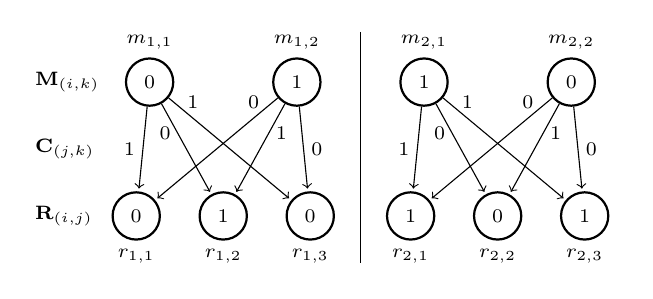
\begin{tikzpicture}[shorten >=1pt,->,draw=black!100, scale=0.85]
	\footnotesize
%	\def \attic{5.95cm}
%	\def \rowtwoht{5.4cm}
%	\def \weightlevel{3.9cm}
%	\def \rowoneht{2.4cm}
%	\def \basement{1.8cm}
%	\def \data{1cm}
%	\def \china{0cm}

%	\def \attic{5.2cm}
%	\def \rowtwoht{4.6cm}
%	\def \weightlevel{3.5cm}
%	\def \rowoneht{2.4cm}
%	\def \basement{1.8cm}
%	\def \data{1cm}
%	\def \china{0cm}

	\def \attic{5cm}
	\def \rowtwoht{4.4cm}
	\def \weightlevel{3.4cm}
	\def \rowoneht{2.4cm}
	\def \basement{1.8cm}
	\def \data{1cm}
	\def \china{0cm}
		
%	\def \attic{5.4cm}
%	\def \rowtwoht{5cm}
%	\def \weightlevel{3.9cm}
%	\def \rowoneht{2.4cm}
%	\def \basement{1.8cm}
%	\def \data{1cm}
%	\def \china{0cm}
	
	\scriptsize
	\tikzstyle{m-node}=[circle,draw=black!100,thick,inner sep=0pt,minimum size=6mm]
	\tikzstyle{r-node}=[circle,draw=black!100,thick,inner sep=0pt,minimum size=6mm]
	\tikzstyle{d-node}=[circle,draw=black!100,fill=gray!45,thick,inner sep=0pt,minimum size=6mm]
	\tikzstyle{annot}=[text width=2.5em]
	% labels
	\tikzstyle{label}=[text width=3em, text centered]
	\tikzstyle{formula}=[text width=30em, text centered]
	\node[annot] (hidden-layer) at (0cm,\rowtwoht) {$\mathbf{M}_{(i,k)}$};
	\node[annot] (weights) at (0cm,\weightlevel) {$\mathbf{C}_{(j,k)}$};
	\node[annot] (r-layer) at (0cm,\rowoneht) {$\mathbf{R}_{(i,j)}$};
	
	\node[m-node] 	(m00)	at (1.3cm,\rowtwoht)		{$0$};
	\node[m-node] 	(m01)	at (3.5cm,\rowtwoht)		{$1$};
	\node[m-node] 	(m10)	at (5.4cm,\rowtwoht) 	{$1$};
	\node[m-node] 	(m11)	at (7.6cm,\rowtwoht)	 	{$0$};
	% \node[m-node] 	(m20)	at (9.65cm,\rowtwoht) 	{$1$};
	% \node[m-node] 	(m21)	at (11.55cm,\rowtwoht)	 	{$1$};
	
	\node[label]	(ml00) 	at (1.3cm,\attic)		{$m_{1,1}$};
	\node[label]	(ml01) 	at (3.5cm,\attic)		{$m_{1,2}$};
	\node[label] 	(ml10)	at (5.4cm,\attic) 	{$m_{2,1}$};
	\node[label] 	(ml11)	at (7.6cm,\attic)	 	{$m_{2,2}$};
	% \node[label] 	(ml20)	at (9.65cm,\attic) 	{$m_{3,1}$};
	% \node[label] 	(ml21)	at (11.55cm,\attic)	 	{$m_{3,2}$};
	
	%\node[m-node] 	(m20)	[right of=m11,xshift=2cm]	 	{$1.0$};
	%\node[m-node] 	(m21)	[right of=m20,xshift=0.5cm]	 	{$1.0$};	
	% reconstructed vector
	\node[r-node] 	(r00)	at (1.1cm,\rowoneht)		{$0$};
	\node[label] 	(rl00)	at (1.1cm,\basement)		{$r_{1,1}$};
	\node[r-node] 	(r01)	at (2.4cm,\rowoneht)		{$1$};
	\node[label] 	(rl01)	at (2.4cm,\basement)		{$r_{1,2}$};
	\node[r-node] 	(r02)	at (3.7cm,\rowoneht)	 	{$0$};
	\node[label] 	(rl02)	at (3.7cm,\basement)	 	{$r_{1,3}$};
	
	\node[r-node] 	(r10)	at (5.2cm,\rowoneht) 		{$1$};
	\node[label] 	(rl10)	at (5.2cm,\basement) 		{$r_{2,1}$};
	\node[r-node] 	(r11) 	at (6.5cm,\rowoneht)   		{$0$};
	\node[label] 	(rl11) 	at (6.5cm,\basement)   		{$r_{2,2}$};
	\node[r-node] 	(r12)	at (7.8cm,\rowoneht)		{$1$};
	\node[label] 	(rl12)	at (7.8cm,\basement)		{$r_{2,3}$};
	
	% \node[r-node] 	(r20) 	at (9.3cm,\rowoneht)  		{$1$};
	% \node[label] 	(rl20) 	at (9.3cm,\basement)  		{$r_{3,1}$};
	% \node[r-node] 	(r21)	at (10.6cm,\rowoneht) 		{$1$};
	% \node[label] 	(rl21)	at (10.6cm,\basement) 		{$r_{3,2}$};
	% \node[r-node] 	(r22) 	at (11.9cm,\rowoneht)   		{$1$};
	% \node[label] 	(rl22) 	at (11.9cm,\basement)   		{$r_{3,3}$};
	
	\draw[-] (4.45cm, \attic+1.5mm) -- (4.45cm, \basement-1.5mm);
%	\draw[-] (8.55cm, \attic+1.5mm) -- (8.55cm, \basement-1.5mm);

	\path
		(m00)	edge	node [left] 	{$1$}	(r00)
		(m00)	edge	node [left,xshift=-1mm,yshift=2mm]	{$0$}	(r01)
		(m00)	edge	node [left,xshift=-3mm,yshift=6mm]	{$1$}	(r02)

		(m01)	edge	node [right,xshift=3mm,yshift=6mm]	{$0$}	(r00)
		(m01)	edge	node [right,xshift=1mm,yshift=2mm]	{$1$}	(r01)
		(m01)	edge	node [right]	{$0$}	(r02)
		%
		(m10)	edge	node [left] 	{$1$}	(r10)
		(m10)	edge	node [left,xshift=-1mm,yshift=2mm]	{$0$}	(r11)
		(m10)	edge	node [left,xshift=-3mm,yshift=6mm] {$1$}	(r12)
		
		(m11)	edge	node [right,xshift=3mm,yshift=6mm]	{$0$}	(r10)
		(m11)	edge	node [right,xshift=1mm,yshift=2mm]	{$1$}	(r11)
		(m11)	edge	node [right]	{$0$}	(r12);
		%
		% (m20)	edge	node [left]	{$1$}	(r20)
		% (m20)	edge	node [left,xshift=-1mm,yshift=4mm]	{$0$}	(r21)
		% (m20)	edge	node [left,xshift=-3mm,yshift=10mm]	{$1$} (r22)
		
		% (m21)	edge	node [right,xshift=3mm,yshift=10mm]		{$0$}	(r20)
		% (m21)	edge	node [right,xshift=1mm,yshift=4mm]{$1$}	(r21)
		% (m21)	edge	node [right]	{$0$}	(r22);		
\end{tikzpicture}
\label{fig:example:subfig2}
}

\begin{framed}
	\centering
	\small
	where
	$\begin{aligned}
	   r_{i,j} = 1 - \Pi_{k=1}^{K} (1 - m_{i,k}c_{j,k}) 
	\end{aligned}$
        \hspace{2em}
        [\textsc{noisy-or} function]
\end{framed}

\end{center}
\caption{A simple MCMM example} % showing learning in progress}
\label{fig:example}
\end{figure}

We can see that while learning is in progress, the cluster activities
($m_{i,k}$) and the cluster centers ($c_{j,k}$) are in flux, as the
error rate is being reduced, but that they converge to values of 0 and
1.  At convergence, a reconstruction node ($r_{i,j}$) is 1 if at least one
$m_{i,k}c_{j,k} = 1$ (and 0 otherwise).

%the activities and the centers are 1 and are 0 otherwise.

% \begin{figure*}[htb]
% \usetikzlibrary{positioning}
% \begin{center}
% \subfigure[Observed Data]{
% \begin{tikzpicture}[shorten >=1pt,->,draw=black!100]
% 	\scriptsize
% 	\tikzstyle{label}=[text width=3em, text centered]
% 	\tikzstyle{annot}=[text width=2.5em]
% 	\tikzstyle{d-node}=[circle,draw=black!100,fill=gray!45,thick,inner sep=0pt,minimum size=6mm]
	
% 	\def \china{0.6cm}
% 	\def \data{0cm}
	
% 	\node[annot] (d-layer) at (0cm,\data) {$\mathbf{D}_{(i,j)}$};
% 	\draw[-] (4.45cm, \china+1.5mm) -- (4.45cm, \data-4.5mm);
% 	\draw[-] (8.55cm, \china+1.5mm) -- (8.55cm, \data-4.5mm);
% 	%\draw[-] (-1cm, \china+.5cm) -- (13cm, \china+.5cm);
% 	%\draw[-] (-1cm, \data-.5cm) -- (13cm, \data-.5cm);
	
% 	\node[label] 	(dl00)	at (1.1cm,\china)		{$d_{1,1}$};
% 	\node[label] 	(dl01)	at (2.4cm,\china)		{$d_{1,2}$};
% 	\node[label] 	(dl02)	at (3.7cm,\china)	 	{$d_{1,3}$};
	
% 	\node[label] 	(dl10)	at (5.2cm,\china) 		{$d_{2,1}$};
% 	\node[label] 	(dl11) 	at (6.5cm,\china)   	{$d_{2,2}$};
% 	\node[label] 	(dl12)	at (7.8cm,\china)		{$d_{2,3}$};
	
% 	\node[label] 	(dl20) 	at (9.3cm,\china)  		{$d_{3,1}$};
% 	\node[label] 	(dl21)	at (10.6cm,\china) 		{$d_{3,2}$};
% 	\node[label] 	(dl22) 	at (11.9cm,\china)   	{$d_{3,3}$};
	
% 	\node[d-node] 	(d00)	at (1.1cm,\data)		{$0$};
% 	\node[d-node] 	(d01)	at (2.4cm,\data)		{$1$};
% 	\node[d-node] 	(d02)	at (3.7cm,\data)		{$0$};

% 	\node[d-node] 	(d10)	at (5.2cm,\data)		{$1$};
% 	\node[d-node] 	(d11)	at (6.5cm,\data)		{$0$};
% 	\node[d-node] 	(d12)	at (7.8cm,\data)		{$1$};
	
% 	\node[d-node] 	(d20)	at (9.3cm,\data)		{$1$};
% 	\node[d-node] 	(d21)	at (10.6cm,\data)		{$1$};
% 	\node[d-node] 	(d22)	at (11.9cm,\data)		{$1$};
% \end{tikzpicture}
% \label{fig:example:subfig0}
% }
% \end{center}

% \usetikzlibrary{positioning}
% %\begin{minipage}{.3\textwidth}
% \begin{center}
% \subfigure[Learning in Progress]{
% \begin{tikzpicture}[shorten >=1pt,->,draw=black!100]
% 	\footnotesize
% 	\def \attic{5.95cm}
% 	\def \rowtwoht{5.4cm}
% 	\def \weightlevel{3.9cm}
% 	\def \rowoneht{2.4cm}
% 	\def \basement{1.8cm}
% 	\def \data{1cm}
% 	\def \china{0cm}
	
% 	\tikzstyle{m-node}=[circle,draw=black!100,thick,inner sep=0pt,minimum size=6mm]
% 	\tikzstyle{r-node}=[circle,draw=black!100,thick,inner sep=0pt,minimum size=6mm]
% 	\tikzstyle{d-node}=[circle,draw=black!100,fill=gray!45,thick,inner sep=0pt,minimum size=6mm]
% 	%\tikzstyle{dots}=[text width=5ex, text centered]
% 	\tikzstyle{annot}=[text width=2.5em]
% 	% labels
% 	\tikzstyle{label}=[text width=3em, text centered]
% 	\tikzstyle{formula}=[text width=30em, text centered]
	
% 	\scriptsize
% 	\node[annot] (hidden-layer) at (0cm,\rowtwoht) {$\mathbf{M}_{(i,k)}$};
% 	\node[annot] (weights) at (0cm,\weightlevel) {$\mathbf{C}_{(j,k)}$};
% 	\node[annot] (r-layer) at (0cm,\rowoneht) {$\mathbf{R}_{(i,j)}$};
	
% 	% hidden layer
% 	\scriptsize
% 	\node[m-node] 	(m00)	at (1.45cm,\rowtwoht)		{$.2$};
% 	\node[m-node] 	(m01)	at (3.35cm,\rowtwoht)		{$.9$};
% 	\node[m-node] 	(m10)	at (5.55cm,\rowtwoht) 	{$.8$};
% 	\node[m-node] 	(m11)	at (7.45cm,\rowtwoht)	 	{$.1$};
% 	\node[m-node] 	(m20)	at (9.65cm,\rowtwoht) 	{$.8$};
% 	\node[m-node] 	(m21)	at (11.55cm,\rowtwoht)	 	{$.9$};
	
% 	%\footnotesize
% 	\node[label]	(ml00) 	at (1.45cm,\attic)		{$m_{1,1}$}; %1.75 -> 1.45
% 	\node[label]	(ml01) 	at (3.35cm,\attic)		{$m_{1,2}$}; %3.05 -> 3.35
% 	\node[label] 	(ml10)	at (5.55cm,\attic) 	{$m_{2,1}$};     %5.85 -> 5.55
% 	\node[label] 	(ml11)	at (7.45cm,\attic)	 	{$m_{2,2}$}; %7.15 -> 7.45
% 	\node[label] 	(ml20)	at (9.65cm,\attic) 	{$m_{3,1}$};     %9.95 -> 9.65
% 	\node[label] 	(ml21)	at (11.55cm,\attic)	 	{$m_{3,2}$}; %11.25 -> 11.55
	
% 	\scriptsize
% 	\node[r-node] 	(r00)	at (1.1cm,\rowoneht)		{$.24$};
% 	\node[r-node] 	(r01)	at (2.4cm,\rowoneht)		{$.81$};
% 	\node[r-node] 	(r02)	at (3.7cm,\rowoneht)	 	{$.23$};
	
% 	\node[r-node] 	(r10)	at (5.2cm,\rowoneht) 		{$.68$};
% 	\node[r-node] 	(r11) 	at (6.5cm,\rowoneht)   	{$.16$};
% 	\node[r-node] 	(r12)	at (7.8cm,\rowoneht)		{$.76$};
	
% 	\node[r-node] 	(r20) 	at (9.3cm,\rowoneht)  		{$.71$};
% 	\node[r-node] 	(r21)	at (10.6cm,\rowoneht) 		{$.83$};
% 	\node[r-node] 	(r22) 	at (11.9cm,\rowoneht)   	{$.77$};
	
% 	\node[label] 	(rl00)	at (1.1cm,\basement)		{$r_{1,1}$};
% 	\node[label] 	(rl01)	at (2.4cm,\basement)		{$r_{1,2}$};
% 	\node[label] 	(rl02)	at (3.7cm,\basement)	 	{$r_{1,3}$};
	
% 	\node[label] 	(rl10)	at (5.2cm,\basement) 		{$r_{2,1}$};
% 	\node[label] 	(rl11) 	at (6.5cm,\basement)   	{$r_{2,2}$};
% 	\node[label] 	(rl12)	at (7.8cm,\basement)		{$r_{2,3}$};
	
% 	\node[label] 	(rl20) 	at (9.3cm,\basement)  		{$r_{3,1}$};
% 	\node[label] 	(rl21)	at (10.6cm,\basement) 		{$r_{3,2}$};
% 	\node[label] 	(rl22) 	at (11.9cm,\basement)   	{$r_{3,3}$};

% 	\draw[-] (4.45cm, \attic+1.5mm) -- (4.45cm, \basement-1.5mm);
% 	\draw[-] (8.55cm, \attic+1.5mm) -- (8.55cm, \basement-1.5mm);

% 	\scriptsize
% 	\path
% 		(m00)	edge	node [left] 	{$.85$}	(r00)
% 		(m00)	edge	node [left,xshift=-1mm,yshift=4mm]	{$.1$}	(r01)
% 		(m00)	edge	node [left,xshift=-1mm,yshift=10mm]	{$.95$}	(r02)

% 		(m01)	edge	node [right,xshift=3mm,yshift=10mm]	{$.1$}	(r00)
% 		(m01)	edge	node [right,xshift=1mm,yshift=4mm]	{$.9$}	(r01)
% 		(m01)	edge	node [right]	{$.05$}	(r02)
% 		%
% 		(m10)	edge	node [left] 	{$.85$}	(r10)
% 		(m10)	edge	node [left,xshift=-1mm,yshift=4mm]	{$.1$}	(r11)
% 		(m10)	edge	node [left,xshift=-1mm,yshift=10mm] {$.95$}	(r12)
		
% 		(m11)	edge	node [right,xshift=3mm,yshift=10mm]	{$.1$}	(r10)
% 		(m11)	edge	node [right,xshift=1mm,yshift=4mm]	{$.9$}	(r11)
% 		(m11)	edge	node [right]	{$.05$}	(r12)
% 		%
% 		(m20)	edge	node [left]	{$.85$}	(r20)
% 		(m20)	edge	node [left,xshift=-1mm,yshift=4mm]	{$.1$}	(r21)
% 		(m20)	edge	node [left,xshift=-1mm,yshift=10mm]	{$.95$} (r22)
		
% 		(m21)	edge	node [right,xshift=3mm,yshift=10mm]		{$.1$}	(r20)
% 		(m21)	edge	node [right,xshift=1mm,yshift=4mm]{$.9$}	(r21)
% 		(m21)	edge	node [right]	{$.05$}	(r22);		
		
% \end{tikzpicture}
% \label{fig:example:subfig1}
% }
% \subfigure[Convergence]{

% \begin{tikzpicture}[shorten >=1pt,->,draw=black!100]
% 	\footnotesize
% 	\def \attic{5.95cm}
% 	\def \rowtwoht{5.4cm}
% 	\def \weightlevel{3.9cm}
% 	\def \rowoneht{2.4cm}
% 	\def \basement{1.8cm}
% 	\def \data{1cm}
% 	\def \china{0cm}
	
% 	\scriptsize
% 	\tikzstyle{m-node}=[circle,draw=black!100,thick,inner sep=0pt,minimum size=6mm]
% 	\tikzstyle{r-node}=[circle,draw=black!100,thick,inner sep=0pt,minimum size=6mm]
% 	\tikzstyle{d-node}=[circle,draw=black!100,fill=gray!45,thick,inner sep=0pt,minimum size=6mm]
% 	\tikzstyle{annot}=[text width=2.5em]
% 	% labels
% 	\tikzstyle{label}=[text width=3em, text centered]
% 	\tikzstyle{formula}=[text width=30em, text centered]
% 	\node[annot] (hidden-layer) at (0cm,\rowtwoht) {$\mathbf{M}_{(i,k)}$};
% 	\node[annot] (weights) at (0cm,\weightlevel) {$\mathbf{C}_{(j,k)}$};
% 	\node[annot] (r-layer) at (0cm,\rowoneht) {$\mathbf{R}_{(i,j)}$};
	
% 	\node[m-node] 	(m00)	at (1.45cm,\rowtwoht)		{$0$};
% 	\node[m-node] 	(m01)	at (3.35cm,\rowtwoht)		{$1$};
% 	\node[m-node] 	(m10)	at (5.55cm,\rowtwoht) 	{$1$};
% 	\node[m-node] 	(m11)	at (7.45cm,\rowtwoht)	 	{$0$};
% 	\node[m-node] 	(m20)	at (9.65cm,\rowtwoht) 	{$1$};
% 	\node[m-node] 	(m21)	at (11.55cm,\rowtwoht)	 	{$1$};
	
% 	\node[label]	(ml00) 	at (1.45cm,\attic)		{$m_{1,1}$};
% 	\node[label]	(ml01) 	at (3.35cm,\attic)		{$m_{1,2}$};
% 	\node[label] 	(ml10)	at (5.55cm,\attic) 	{$m_{2,1}$};
% 	\node[label] 	(ml11)	at (7.45cm,\attic)	 	{$m_{2,2}$};
% 	\node[label] 	(ml20)	at (9.65cm,\attic) 	{$m_{3,1}$};
% 	\node[label] 	(ml21)	at (11.55cm,\attic)	 	{$m_{3,2}$};
	
% 	%\node[m-node] 	(m20)	[right of=m11,xshift=2cm]	 	{$1.0$};
% 	%\node[m-node] 	(m21)	[right of=m20,xshift=0.5cm]	 	{$1.0$};	
% 	% reconstructed vector
% 	\node[r-node] 	(r00)	at (1.1cm,\rowoneht)		{$0$};
% 	\node[label] 	(rl00)	at (1.1cm,\basement)		{$r_{1,1}$};
% 	\node[r-node] 	(r01)	at (2.4cm,\rowoneht)		{$1$};
% 	\node[label] 	(rl01)	at (2.4cm,\basement)		{$r_{1,2}$};
% 	\node[r-node] 	(r02)	at (3.7cm,\rowoneht)	 	{$0$};
% 	\node[label] 	(rl02)	at (3.7cm,\basement)	 	{$r_{1,3}$};
	
% 	\node[r-node] 	(r10)	at (5.2cm,\rowoneht) 		{$1$};
% 	\node[label] 	(rl10)	at (5.2cm,\basement) 		{$r_{2,1}$};
% 	\node[r-node] 	(r11) 	at (6.5cm,\rowoneht)   		{$0$};
% 	\node[label] 	(rl11) 	at (6.5cm,\basement)   		{$r_{2,2}$};
% 	\node[r-node] 	(r12)	at (7.8cm,\rowoneht)		{$1$};
% 	\node[label] 	(rl12)	at (7.8cm,\basement)		{$r_{2,3}$};
	
% 	\node[r-node] 	(r20) 	at (9.3cm,\rowoneht)  		{$1$};
% 	\node[label] 	(rl20) 	at (9.3cm,\basement)  		{$r_{3,1}$};
% 	\node[r-node] 	(r21)	at (10.6cm,\rowoneht) 		{$1$};
% 	\node[label] 	(rl21)	at (10.6cm,\basement) 		{$r_{3,2}$};
% 	\node[r-node] 	(r22) 	at (11.9cm,\rowoneht)   		{$1$};
% 	\node[label] 	(rl22) 	at (11.9cm,\basement)   		{$r_{3,3}$};
	
% 	\draw[-] (4.45cm, \attic+1.5mm) -- (4.45cm, \basement-1.5mm);
% 	\draw[-] (8.55cm, \attic+1.5mm) -- (8.55cm, \basement-1.5mm);

% 	\path
% 		(m00)	edge	node [left] 	{$1$}	(r00)
% 		(m00)	edge	node [left,xshift=-1mm,yshift=4mm]	{$0$}	(r01)
% 		(m00)	edge	node [left,xshift=-3mm,yshift=10mm]	{$1$}	(r02)

% 		(m01)	edge	node [right,xshift=3mm,yshift=10mm]	{$0$}	(r00)
% 		(m01)	edge	node [right,xshift=1mm,yshift=4mm]	{$1$}	(r01)
% 		(m01)	edge	node [right]	{$0$}	(r02)
% 		%
% 		(m10)	edge	node [left] 	{$1$}	(r10)
% 		(m10)	edge	node [left,xshift=-1mm,yshift=4mm]	{$0$}	(r11)
% 		(m10)	edge	node [left,xshift=-3mm,yshift=10mm] {$1$}	(r12)
		
% 		(m11)	edge	node [right,xshift=3mm,yshift=10mm]	{$0$}	(r10)
% 		(m11)	edge	node [right,xshift=1mm,yshift=4mm]	{$1$}	(r11)
% 		(m11)	edge	node [right]	{$0$}	(r12)
% 		%
% 		(m20)	edge	node [left]	{$1$}	(r20)
% 		(m20)	edge	node [left,xshift=-1mm,yshift=4mm]	{$0$}	(r21)
% 		(m20)	edge	node [left,xshift=-3mm,yshift=10mm]	{$1$} (r22)
		
% 		(m21)	edge	node [right,xshift=3mm,yshift=10mm]		{$0$}	(r20)
% 		(m21)	edge	node [right,xshift=1mm,yshift=4mm]{$1$}	(r21)
% 		(m21)	edge	node [right]	{$0$}	(r22);		
% \end{tikzpicture}
% \label{fig:example:subfig2}
% }

% \begin{framed}
% 	\centering
% 	\small
% 	where
% 	$\begin{aligned}
% 	   r_{i,j} = 1 - \Pi_{k=1}^{K} (1 - m_{i,k}c_{j,k}) 
% 	\end{aligned}$
% \end{framed}

% \label{fig:example}
% \caption{MCMM example showing learning in progress}
% \end{center}
% \end{figure*}

